% schéma
\section{Kernel}
\begin{frame}
	\center{\huge{Noyau}}
	\begin{columns}
	\begin{column}{0.38\linewidth}
		\begin{figure}
			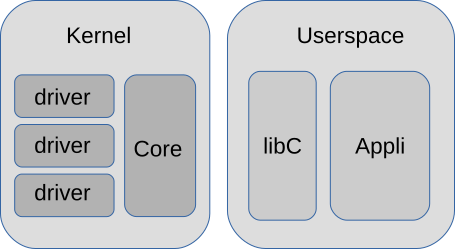
\includegraphics[height=2.5cm]{img/arch_linux_full.png}
			 \caption{kernel}
		\end{figure}
	\end{column}
	\begin{column}{0.60\linewidth}
		\begin{itemize}
			\item<2-> Gère le matériel
			\item<3-> Gère les ressources
			\item<4-> Implémente certains protocoles
			\item<5-> Couche d'abstraction
			\item<6-> Isolé de l'espace utilisateur
			\item<7-> Composant critique
		\end{itemize}
	\end{column}
	\end{columns}
\end{frame}


\begin{frame}
	\center{\huge{Linux}}
	\begin{columns}[t]
		\begin{column}{0.70\textwidth}
			\begin{itemize}
				\item<2-> Beaucoup d'architectures
				\item<3-> Beaucoup de périphériques
				\item<4-> Beaucoup de fonctionnalités
				\item<5-> Communauté active
				\item<6-> Entièrement configurable
				\item<7-> Libre
			\end{itemize}
		\end{column}
		\begin{column}{0.25\textwidth}
			\begin{figure}
				
\includegraphics[height=2cm]{img/tux.png}
				\caption{Tux}
			\end{figure}
		\end{column}
	\end{columns}
	\begin{block}<8->{Variantes}
		\begin{itemize}
			\item<8-> Temps réel : Preempt-RT, xenomai
			\item<9-> Microcontrolleur : uCLinux
			\item<10-> Sécurité : SELinux, grsecurity
		\end{itemize}
	\end{block}
\end{frame}
% choix de la version
\subsection{Drivers}
\begin{frame}
	\center{\huge{Drivers}}
	\begin{itemize}
		\item Support d'un périphérique
		\item Support d'un protocole
		\item Libre ou Propriétaire
	\end{itemize}
	\begin{block}<2->{Kernel module}
		\begin{itemize}
		\item Extension du kernel
		\item Intégration statique ou dynamique
		\item \textbf{Lié à une version du kernel}
		\item Gestion des dépendances
		\end{itemize}
	\end{block}
\end{frame}
% drivers, support
\subsection{Configuration}
\begin{frame}[t]
	\center{\huge{Configuration du noyau}}
	\begin{columns}[T]
		\begin{column}{0.50\textwidth}
		\begin{itemize}
			\item Choix des drivers
			\item Choix des fonctionnalités
			\item Options de debug
			\item Options d'optimisation
		\end{itemize}
		\end{column}
		\begin{column}{0.48\textwidth}
			\vspace{-0.2cm}
			\begin{figure}
				\includegraphics<2->[height=3cm]{img/menuconfig.png}
			\end{figure}
		\end{column}
	\end{columns}
	\begin{block}<2->{Kconfig}
		\begin{itemize}
			\item Plusieurs UI
			\item Dépendances entre options
			\item Génère un fichier de conf
		\end{itemize}
	\end{block}
\end{frame}
% choix des options : selon matos, contraintes
